%!TEX root = ../../lod-group1.tex
%\subsection{Matching}
\label{subsec_evaluation_matching}

\subsection{Introduction}
The matching algorithm, explained in \ref{subsec_method_matching}, depends on multiple parameters.
The following paragraphs explain the process of tuning these parameters and evaluating the quality of the matching algorithm.

Evaluation is done on two sets of 4000 randomly selected movies.
The selection is done by listing all movies sorted by name and then using $Random.shuffle$ to shuffle the list and take the first 4000 movies.
The first list is used for the parameter optimization, while the second is used for the final evaluation.
To get a gold standard only those movies with an annotated IMDb-id are taken into consideration.
However, the id is not used to match the movies, it is only used as the gold standard.
These movies can be split into two parts: the movies that could potentially be matched and the movies that cannot be matched, i.e. movies that do not exist in the database.
The result is a list of around 3300 movies the algorithm is tested with.
2008 of these movies could possibly be matched.

Evaluation itself is done by means of precision, recall and F0.5-measure.
As explained in Section \ref{subsec_method_matching}, Precision is more important and therefore the F0.5-measure is additionally observed in the evaluation process.
The following paragraphs show the definitions of the relevant sets for the purpose of calculating these evaluation metrics.

Given the set of new movies $N$ and the set of existing movies $M$ the following function returns the correct matching movie $m_{j} \in M$ of a new movie $n_{i} \in N$:

\begin{align}
	gold: ~&N \rightarrow M \cup \{\bot\} \\
	gold(n) &=
		\begin{cases}
		m \in M ~\text{if matching movie m exists in database}  \\
		\bot
		\end{cases}
\end{align}

The function $gold$ is defined by looking at the IMDb-ids as described above.
Using this function and the algorithm $match_{n_{i}}$ explained in \ref{subsec_method_matching} the following sets are defined:

\begin{description}
\item[True Positives (TP)] is the set of correct matches between a new movie and an existing one in the database,
\begin{align}
TP &\coloneqq \Set*{(n_i, match(n_i))}{match(n_i) = gold(n_i) \land match(n_i) \neq \bot}
\end{align}
\item[False Positives (FP)] is the set of incorrect matches, either meaning another movie is the correct match or no correct match exists in the database
\begin{align}
FP &\coloneqq \Set*{(n_i, match(n_i))}{match(n_i) \neq gold(n_i) \land match(n_i) \neq \bot}
\end{align}\item[True Negatives (TN)] is the set of tuples that are no matches and that cannot be matched because they are not in the database,
\begin{align}
FP &\coloneqq \Set*{(n_i, m_j)}{m_j \in M \land (m_j \neq match(n_i) \land m_j \neq gold(n_i) \lor m_j = \bot)}
\end{align}
\item[False Negatives (FN)] is the set of correct matches between movies that have not been found.
\begin{align}
FP &\coloneqq \Set*{(n_i, m_j)}{m_j \in M \land m_j \neq match(n_i) \land m_j = gold(n_i) \land m_j \neq \bot}
\end{align}
\end{description}

Based on these sets, standard definitions of the evaluation metrics precision, recall, F0.5-measure are used.

To generate consistent results, the whole evaluation is done without the distributed enviroment, as explained in section \ref{subsec_method_architecture}, but on a single machine with the following system specifications:
\begin{itemize}
	\item CPU: Pentium(R) Dual-Core  CPU E5300  @ 2.60GHz
	\item RAM: 16GB, Java is run with 4GB of RAM
	\item OS: Debian 3.2.57
\end{itemize}

The evaluation process is structured into two parts: parameter optimization and final evaluation.
In the first part, several experiments are conducted regarding the optimal parameters.
Concretely, the goal was to find good values for $ACT\_DIST$, $MIN\_SCORE$ and $CANDIDATE\_SET\_SIZE$.


The Levenshtein distance of the candidates is regared in the third test.
Finally, the algorithm will be evaluated on the second dataset against the baseline approach of matching by name.
Thereby each annotated name of the movie is compared with each name of all the movies in the database.

what is evaluated TODO
list of annotated properties
TODO: Important, how are the other parameters set?

\subsection{$CANDIDATE\_SET\_SIZE$ parameter}
Therefore, the first test looks at the impact on the quality of the results when the number of considered candidates is lowered.

\begin{figure}[h!]
  \begin{center}
  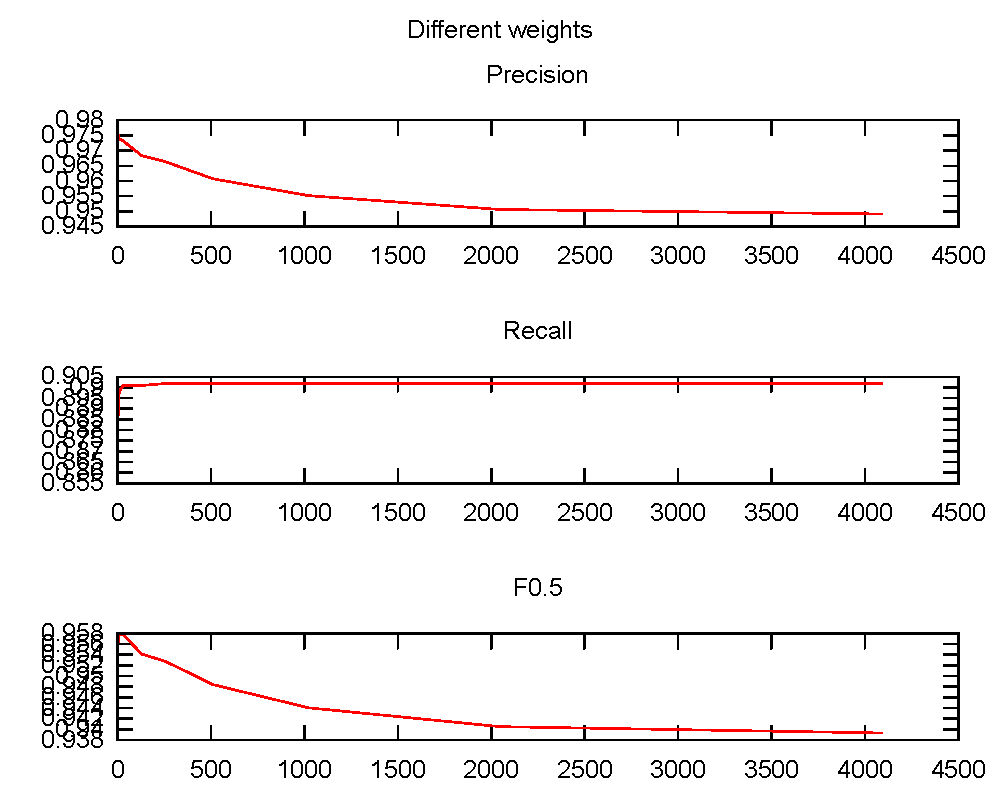
\includegraphics[width=0.8\textwidth]{images/candidateSetSize.pdf}
  \end{center}
  \caption{TODO}
  \label{fig_candidate_set_size}
\end{figure}

\subsection{Threshold Parameter}

A second test observes the maximum Levenshtein distance between two actors and the threshold that needs to be reached for the actor overlap.


\subsection{Refinement Weight}

\begin{figure}[h!]
  \begin{center}
  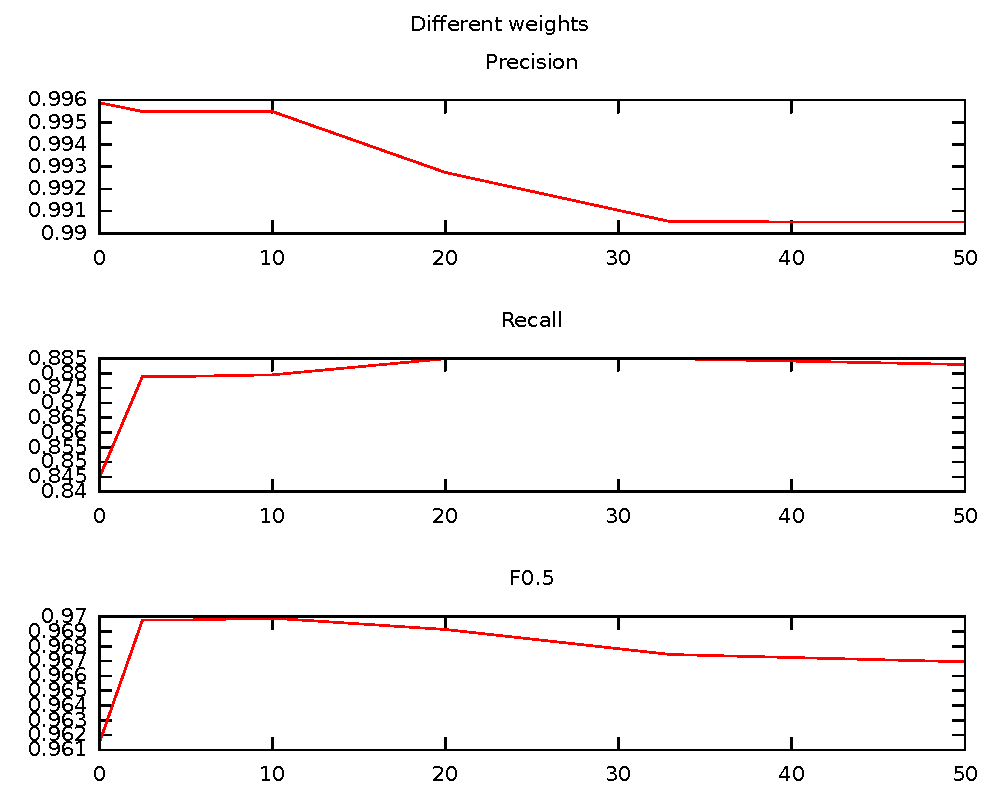
\includegraphics[width=0.8\textwidth]{images/graph_weight.pdf}
  \end{center}
  \caption{TODO}
  \label{fig_weight}
\end{figure}
\subsection{Final evaluation}
With the determined parameters:
TODO: Write final parameters
the final performance of the matching algorithm is illustrated in figure ref

Comparison to Baseline Approach

\begin{figure}[h!]
  \begin{center}
  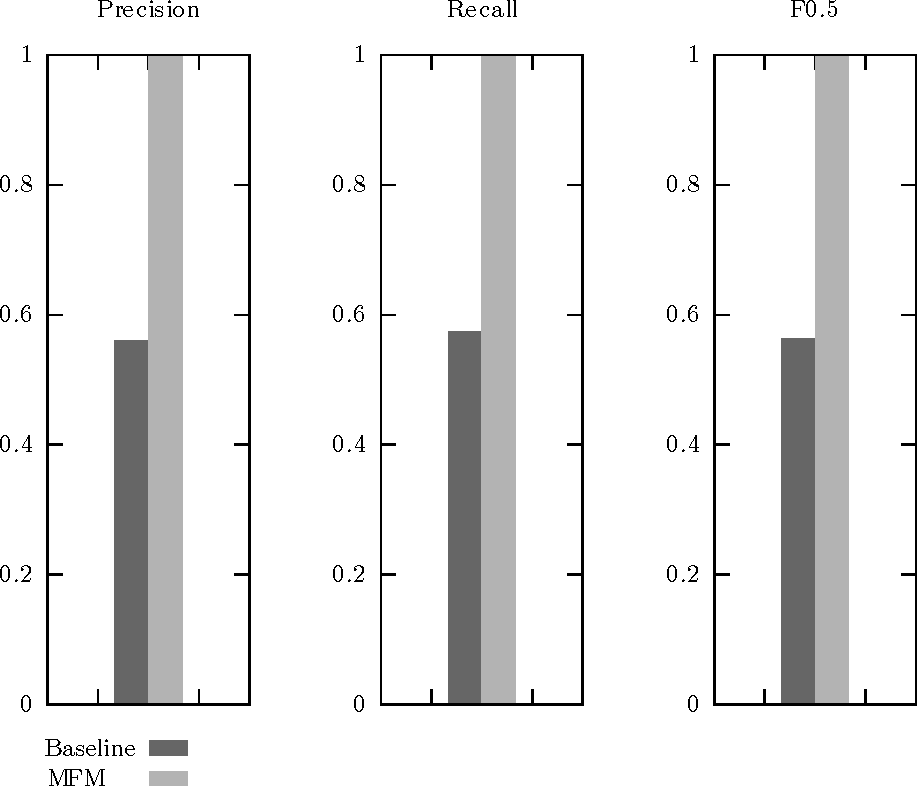
\includegraphics[width=0.8\textwidth]{images/baseline.pdf}
  \end{center}
  \caption{TODO}
  \label{fig_baseline}
\end{figure}

\subsection{Error sources}
What is wrong for incorrectly matchedm
and what is wrong for not matcheds that should be matched?